\documentclass{standalone}
\usepackage{tikz}
\usepackage{ctex,siunitx,ninecolors}
\setCJKmainfont{Noto Serif CJK SC}
\usepackage{tkz-euclide}
\usepackage{amsmath}
\usetikzlibrary{patterns, calc}
\usetikzlibrary {decorations.pathmorphing, decorations.pathreplacing, decorations.shapes,}
\begin{document}
\small
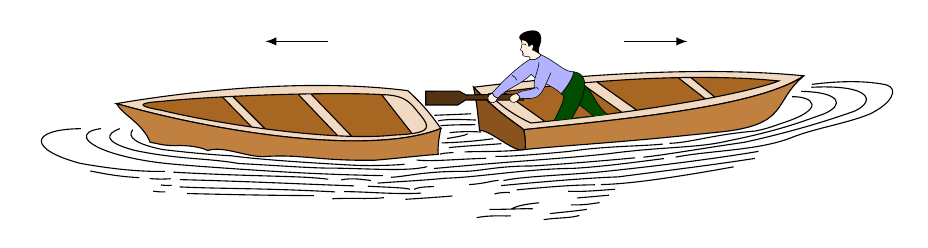
\begin{tikzpicture}[>=latex,scale=0.8]
  % \useasboundingbox(-2.4,-0.4)rectangle(2.4,0.6);
  \draw( 0.872,1.815)..controls( 0.036,1.805)and( 0.037,1.483)..
  ( 0.862,1.264)..controls( 1.531,1.145)and( 1.926,1.133)..( 2.206,1.136)
  ( 1.189,1.816)..controls( 0.824,1.767)and( 0.896,1.580)..
  ( 1.376,1.428)..controls( 1.887,1.273)and( 2.324,1.253)..
  ( 2.721,1.220)..controls( 3.917,1.133)and( 4.636,1.089)..( 5.664,1.069)
  ( 6.368,1.211)..controls( 6.045,1.133)and( 5.495,1.180)..
  ( 4.900,1.188)..controls( 4.574,1.185)and( 4.090,1.224)..
  ( 3.378,1.262)..controls( 2.867,1.351)and( 2.421,1.324)..
  ( 1.727,1.470)..controls( 1.219,1.602)and( 1.264,1.735)..( 1.491,1.815)
  ( 1.698,1.799)..controls( 1.595,1.689)and( 1.735,1.569)..
  ( 2.178,1.482)..controls( 2.522,1.443)and( 2.852,1.407)..
  ( 3.260,1.384)..controls( 3.623,1.334)and( 4.315,1.283)..
  ( 5.121,1.239)..controls( 5.395,1.220)and( 5.797,1.231)..( 6.012,1.249)
  ( 6.482,2.027)..controls( 6.673,2.035)and( 6.867,2.041)..( 7.065,2.051)
  ( 6.543,1.939)..controls( 6.690,1.971)and( 6.901,1.961)..( 7.143,1.952)
  ( 6.581,1.862)..controls( 6.804,1.879)and( 6.969,1.877)..( 7.134,1.878)
  ( 6.725,1.750)..controls( 6.877,1.771)and( 7.078,1.772)..( 7.226,1.761)
  ( 6.686,1.659)..controls( 6.846,1.685)and( 6.971,1.707)..( 7.012,1.732)
  ( 6.600,1.589)..controls( 6.921,1.595)and( 7.268,1.633)..( 7.417,1.656)
  ( 6.714,1.514)..controls( 7.050,1.548)and( 7.320,1.556)..( 7.548,1.577)
  ( 6.965,1.446)..controls( 7.274,1.457)and( 7.639,1.445)..( 7.925,1.486)
  ( 6.787,1.436)..controls( 6.659,1.428)and( 6.603,1.423)..( 6.575,1.409)
  ( 7.306,1.345)..controls( 6.745,1.326)and( 6.450,1.291)..( 6.201,1.317)
  ( 7.453,1.374)..controls( 7.742,1.368)and( 8.520,1.444)..
  ( 8.634,1.455)..controls( 9.184,1.539)and( 9.794,1.537)..(10.109,1.570)
  (12.161,2.322)..controls(12.486,2.330)and(12.740,2.132)..
  (11.983,1.896)..controls(11.874,1.856)and(11.722,1.803)..
  (11.572,1.777)..controls(10.892,1.718)and(10.543,1.591)..(10.216,1.582)
  (12.304,2.407)..controls(12.925,2.396)and(13.011,2.196)..
  (12.664,2.048)..controls(12.341,1.935)and(11.978,1.788)..
  (11.156,1.623)..controls(10.674,1.505)and(10.119,1.532)..
  ( 9.264,1.419)..controls( 8.515,1.336)and( 7.761,1.302)..( 6.478,1.182)
  (12.468,2.472)..controls(13.424,2.518)and(13.494,2.253)..
  (13.156,2.094)..controls(12.583,1.889)and(11.973,1.724)..
  (11.413,1.600)..controls(10.680,1.493)and(10.129,1.396)..( 9.803,1.362)
  (10.313,1.363)..controls(10.865,1.470)and(11.634,1.467)..
  (12.153,1.673)..controls(12.519,1.821)and(13.049,1.901)..
  (13.406,2.052)..controls(13.747,2.220)and(13.865,2.450)..
  (13.655,2.511)..controls(13.329,2.578)and(12.930,2.575)..(12.476,2.518)
  ( 5.794,1.043)..controls( 6.052,1.055)and( 6.307,1.139)..
  ( 6.945,1.137)..controls( 7.202,1.136)and( 7.487,1.225)..
  ( 8.029,1.222)..controls( 8.500,1.251)and( 8.972,1.288)..( 9.672,1.352)
  ( 5.581,0.950)..controls( 5.931,0.977)and( 6.244,0.988)..
  ( 6.659,1.028)..controls( 7.198,1.044)and( 7.926,1.176)..
  ( 8.695,1.185)..controls( 9.161,1.212)and( 9.726,1.289)..(10.128,1.340)
  ( 1.022,1.143)..controls( 1.334,1.079)and( 1.547,1.050)..( 1.799,1.037)
( 1.962,1.023)..controls( 2.127,1.008)and( 2.246,1.017)..( 2.297,1.020)
( 2.144,0.921)..controls( 2.225,0.910)and( 2.280,0.912)..( 2.312,0.916)
( 2.019,0.823)..controls( 2.097,0.812)and( 2.160,0.808)..( 2.213,0.812)
( 2.339,1.124)..controls( 3.745,1.047)and( 4.356,1.071)..( 4.798,1.012)
( 2.442,1.006)..controls( 3.527,0.979)and( 4.553,0.927)..( 5.210,0.907)
( 2.441,0.890)..controls( 3.179,0.857)and( 3.772,0.872)..( 4.908,0.811)
( 2.557,0.785)..controls( 3.538,0.761)and( 4.061,0.754)..( 4.571,0.752)
( 5.004,1.002)..controls( 5.190,1.039)and( 5.346,1.005)..( 5.477,0.992)
( 5.428,0.901)..controls( 5.843,0.880)and( 6.031,0.876)..( 6.098,0.852)
( 5.049,0.816)..controls( 5.440,0.813)and( 5.908,0.767)..( 6.274,0.792)
( 4.863,0.702)..controls( 5.153,0.717)and( 5.488,0.695)..( 5.683,0.719)
( 6.162,0.852)..controls( 6.219,0.887)and( 6.380,0.895)..( 6.474,0.894)
( 6.022,0.693)..controls( 6.333,0.713)and( 6.622,0.733)..( 6.770,0.746)
( 7.036,0.927)..controls( 7.286,0.942)and( 7.391,0.989)..( 7.503,0.994)
( 7.581,0.990)..controls( 7.844,1.051)and( 8.400,1.070)..
( 9.053,1.122)..controls( 9.780,1.195)and(10.812,1.317)..(11.628,1.454)
(11.572,1.343)..controls(10.858,1.231)and(10.061,1.136)..
( 9.402,1.049)..controls( 9.004,1.039)and( 8.136,0.967)..( 7.542,0.911)
( 7.437,0.778)..controls( 7.523,0.804)and( 7.615,0.803)..( 7.681,0.802)
( 7.703,0.538)..controls( 7.816,0.606)and( 8.026,0.625)..( 8.146,0.638)
( 7.358,0.533)..controls( 7.706,0.533)and( 7.932,0.551)..( 8.048,0.542)
( 7.156,0.403)..controls( 7.382,0.444)and( 7.528,0.425)..( 7.697,0.430)
( 8.605,0.821)..controls( 8.881,0.811)and( 9.096,0.836)..( 9.353,0.853)
( 8.748,0.715)..controls( 8.946,0.730)and( 9.133,0.749)..( 9.254,0.758)
( 8.650,0.606)..controls( 8.819,0.596)and( 9.004,0.624)..( 9.107,0.642)
( 8.316,0.466)..controls( 8.472,0.485)and( 8.683,0.502)..( 8.903,0.533)
( 8.219,0.370)..controls( 8.435,0.405)and( 8.633,0.390)..( 8.786,0.437)
( 7.790,0.843)..controls( 8.536,0.913)and( 8.764,0.920)..( 9.032,0.924)
( 9.125,0.927)..controls( 9.432,0.934)and( 9.957,0.978)..(11.235,1.209);
\draw[fill=brown9](6.587,1.818)..controls(5.496,1.380)and(3.089,1.743)..
(1.436,2.213)..controls(3.276,2.522)and(4.884,2.568)..
(6.061,2.418)..controls(6.344,2.163)and(6.484,1.959)..cycle
( 7.901,1.799)..controls( 7.701,1.956)and( 7.485,2.078)..
( 7.106,2.473)..controls( 9.304,2.738)and(11.064,2.779)..
(12.349,2.654)..controls(11.660,2.189)and( 9.780,1.992)..cycle;
\draw[fill=brown5,even odd rule](5.838,1.713)..controls(4.906,1.606)and(3.039,1.890)..
(2.139,2.109)..controls(1.761,2.175)and(1.772,2.221)..
(2.125,2.246)..controls(3.199,2.353)and(4.986,2.398)..
(5.646,2.355)..controls(5.955,2.348)and(6.066,2.280)..
(6.202,2.103)..controls(6.410,1.853)and(6.516,1.741)..(5.838,1.713)
(5.646,2.355)..controls(5.955,2.348)and(6.066,2.280)..
(6.202,2.103)..controls(6.373,1.898)and(6.475,1.785)..(6.130,1.736)--cycle
(4.950,1.701)--(4.319,2.364)--(4.524,2.367)--(5.173,1.692)--cycle
(3.586,1.840)--(3.117,2.319)--(3.281,2.327)--(3.796,1.812)--cycle
( 8.015,1.905)..controls( 7.779,2.014)and( 7.555,2.157)..
( 7.350,2.368)..controls( 9.197,2.632)and(10.842,2.686)..
(11.952,2.572)..controls(11.393,2.361)and( 9.762,2.075)..cycle
( 9.696,2.108)--( 9.059,2.559)--( 8.807,2.538)--( 9.461,2.075)
(10.786,2.287)--(10.351,2.625)--(10.552,2.628)--(10.936,2.316)
(7.573,2.399)--(7.350,2.368)..controls(7.555,2.157)and(7.779,2.014)..(8.015,1.905)--(8.239,1.928)--cycle;
\draw[fill=brown](1.436,2.213)..controls(1.541,2.029)and(1.848,1.904)..
(1.973,1.598)..controls(2.074,1.586)and(2.180,1.537)..
(2.419,1.547)..controls(2.681,1.549)and(2.829,1.497)..
(2.885,1.468)..controls(3.136,1.544)and(3.462,1.376)..
(3.763,1.370)..controls(4.354,1.417)and(4.642,1.299)..
(5.543,1.314)..controls(5.969,1.350)and(6.382,1.401)..
(6.546,1.406)..controls(6.532,1.483)and(6.552,1.666)..
(6.587,1.818)..controls(5.496,1.380)and(3.089,1.743)..cycle
(11.003,1.760)..controls(12.131,1.874)and(11.848,2.238)..
(12.349,2.654)..controls(11.660,2.189)and( 9.780,1.992)..
( 7.901,1.799)..controls( 7.930,1.643)and( 7.933,1.581)..
( 7.923,1.484)..controls( 8.443,1.538)and( 9.090,1.574)..(10.079,1.667)--cycle;
\draw[fill=brown4](7.923,1.484)..controls(7.933,1.581)and(7.930,1.643)..
(7.901,1.799)..controls(7.701,1.956)and(7.485,2.078)..
(7.106,2.473)..controls(7.162,2.201)and(7.178,1.992)..
(7.200,1.789)..controls(7.396,1.786)and(7.758,1.413)..cycle;
\draw[fill=brown2](7.899,2.268)--(7.892,2.367)--(6.988,2.349)--(6.875,2.411)--(6.347,2.409)--(6.347,2.191)--(6.856,2.191)--(6.980,2.270)--cycle;
\draw[fill=green!30!black,very thin,even odd rule](9.235,2.038)..controls(9.054,2.180)and(9.002,2.393)..
(8.871,2.502)..controls(8.875,2.688)and(8.739,2.717)..
(8.693,2.718)..controls(8.694,2.630)and(8.568,2.450)..
(8.495,2.370)..controls(8.564,2.349)and(8.552,2.272)..(8.383,1.943)
(9.013,2.005)..controls(8.928,2.084)and(8.850,2.145)..
(8.782,2.194)..controls(8.747,2.120)and(8.701,2.035)..(8.66,1.97);
\draw[fill=pink!10!orange!10,very thin]
(7.788,2.371)..controls(7.568,2.331)and(7.733,2.126)..
(7.837,2.301)..controls(7.845,2.327)and(7.824,2.351)..(7.788,2.371)
(7.488,2.299)..controls(7.449,2.320)and(7.408,2.334)..
(7.403,2.383)..controls(7.227,2.303)and(7.427,2.126)..(7.488,2.299)
(8.181,2.986)..controls(8.126,3.007)and(8.092,3.059)..
(8.041,3.064)..controls(8.084,3.149)and(8.031,3.183)..
(7.985,3.121)..controls(7.974,3.206)and(7.913,3.233)..
(7.859,3.222)..controls(7.913,3.128)and(7.823,3.072)..
(7.862,3.049)..controls(7.920,3.053)and(7.845,3.014)..
(7.897,3.008)..controls(7.859,2.978)and(7.910,2.958)..
(7.948,2.958)..controls(8.009,2.965)and(8.012,2.936)..
(7.997,2.914)..controls(8.052,2.895)and(8.127,2.917)..(8.181,2.986);
\fill(7.904,3.344)..controls(8.089,3.418)and(8.254,3.369)..
(8.144,3.094)..controls(8.136,3.020)and(8.144,3.002)..
(8.181,2.986)..controls(8.126,3.007)and(8.092,3.059)..
(8.041,3.064)..controls(8.084,3.149)and(8.031,3.183)..
(7.985,3.121)..controls(7.974,3.206)and(7.913,3.233)..
(7.859,3.222)..controls(7.805,3.251)and(7.824,3.300)..cycle;
\draw[fill=blue!30!white,very thin]
(8.495,2.370)..controls(8.353,2.514)and(8.100,2.569)..
(8.022,2.678)..controls(7.844,2.503)and(7.643,2.461)..
(7.488,2.299)..controls(7.449,2.320)and(7.408,2.334)..
(7.403,2.383)..controls(7.623,2.624)and(7.782,2.773)..
(7.997,2.914)..controls(8.052,2.895)and(8.127,2.917)..
(8.181,2.986)..controls(8.438,2.865)and(8.545,2.713)..
(8.693,2.718)..controls(8.694,2.630)and(8.568,2.450)..cycle;
\draw[fill=blue!30!white,very thin](8.144,2.872)..controls(8.137,2.723)and(8.044,2.605)..
(8.073,2.459)..controls(7.981,2.410)and(7.885,2.437)..
(7.788,2.371)..controls(7.824,2.351)and(7.845,2.327)..
(7.837,2.301)..controls(8.165,2.272)and(8.162,2.308)..(8.333,2.702);
\draw[very thin]
(8.871,2.502)..controls(8.869,2.427)and(8.844,2.327)..(8.782,2.194)
(7.884,3.156)..controls(7.913,3.165)and(7.933,3.157)..(7.940,3.140)
(7.713,2.662)..controls(7.755,2.653)and(7.778,2.616)..(7.793,2.584)
(8.073,2.459)..controls(8.112,2.463)and(8.126,2.481)..(8.138,2.438);
\draw[->](9.5,3.2)--++(1,0);
\draw[->](4.8,3.2)--++(-1,0);
  \end{tikzpicture}
\end{document}